% =============================================================================
% UNCASE Whitepaper v2 — March 2026
% Unbiased Neutral Convention for Agnostic Seed Engineering
% =============================================================================
\documentclass[11pt,a4paper,twoside]{article}

% --- Geometry & Layout ---
\usepackage[top=2.5cm, bottom=2.5cm, left=2.5cm, right=2.5cm]{geometry}
\usepackage[parfill]{parskip}
\usepackage{setspace}
\setstretch{1.15}

% --- Typography ---
\usepackage[T1]{fontenc}
\usepackage[utf8]{inputenc}
\usepackage{lmodern}
\usepackage{microtype}

% --- Colors ---
\usepackage[dvipsnames,svgnames,x11names]{xcolor}
\definecolor{uncaseBlue}{HTML}{1E40AF}
\definecolor{uncaseDark}{HTML}{0F172A}
\definecolor{uncaseAccent}{HTML}{3B82F6}
\definecolor{uncaseGreen}{HTML}{059669}
\definecolor{uncaseRed}{HTML}{DC2626}
\definecolor{codeBg}{HTML}{F1F5F9}
\definecolor{tableBg}{HTML}{F8FAFC}
\definecolor{tableHeader}{HTML}{E2E8F0}

% --- Graphics & Figures ---
\usepackage{graphicx}
\usepackage{float}
\usepackage{tikz}
\usetikzlibrary{shapes.geometric, arrows.meta, positioning, calc, fit, backgrounds}

% --- Tables ---
\usepackage{booktabs}
\usepackage{tabularx}
\usepackage{colortbl}
\usepackage{multirow}
\usepackage{array}
\newcolumntype{L}[1]{>{\raggedright\arraybackslash}p{#1}}
\newcolumntype{C}[1]{>{\centering\arraybackslash}p{#1}}
\newcolumntype{R}[1]{>{\raggedleft\arraybackslash}p{#1}}

% --- Code Listings ---
\usepackage{listings}
\lstset{
  backgroundcolor=\color{codeBg},
  basicstyle=\ttfamily\small,
  breaklines=true,
  frame=single,
  framerule=0pt,
  rulecolor=\color{codeBg},
  xleftmargin=1em,
  xrightmargin=1em,
  framexleftmargin=0.5em,
  framexrightmargin=0.5em,
  aboveskip=1em,
  belowskip=1em,
  tabsize=2,
  showstringspaces=false,
  keywordstyle=\color{uncaseBlue}\bfseries,
  commentstyle=\color{gray},
  stringstyle=\color{uncaseGreen},
}

% --- Hyperlinks ---
\usepackage[
  colorlinks=true,
  linkcolor=uncaseBlue,
  citecolor=uncaseBlue,
  urlcolor=uncaseAccent,
  bookmarks=true,
  bookmarksnumbered=true,
]{hyperref}

% --- Headers & Footers ---
\usepackage{fancyhdr}
\pagestyle{fancy}
\fancyhf{}
\fancyhead[LE,RO]{\textcolor{gray}{\small UNCASE Whitepaper v2}}
\fancyhead[RE,LO]{\textcolor{gray}{\small March 2026}}
\fancyfoot[CE,CO]{\textcolor{gray}{\small\thepage}}
\renewcommand{\headrulewidth}{0.4pt}
\renewcommand{\footrulewidth}{0pt}

% --- Section Styling ---
\usepackage{titlesec}
\titleformat{\section}
  {\Large\bfseries\color{uncaseDark}}
  {\thesection}{1em}{}[\vspace{0.3em}\titlerule]
\titleformat{\subsection}
  {\large\bfseries\color{uncaseBlue}}
  {\thesubsection}{0.8em}{}
\titleformat{\subsubsection}
  {\normalsize\bfseries\color{uncaseDark}}
  {\thesubsubsection}{0.6em}{}

% --- Bibliography ---
\usepackage[numbers,sort&compress]{natbib}

% --- Math ---
\usepackage{amsmath,amssymb}

% --- Misc ---
\usepackage{enumitem}
\setlist[itemize]{nosep, leftmargin=1.5em}
\setlist[enumerate]{nosep, leftmargin=1.5em}

% --- Custom Commands ---
\newcommand{\uncase}{\textsc{UNCASE}}
\newcommand{\scsf}{\textsc{SCSF}}
\newcommand{\metric}[1]{\texttt{#1}}
\newcommand{\layer}[1]{\textbf{Layer~#1}}
\newcommand{\highlight}[1]{\colorbox{yellow!20}{#1}}
\newcommand{\cmark}{\textcolor{uncaseGreen}{\checkmark}}
\newcommand{\xmark}{\textcolor{uncaseRed}{$\times$}}

% =============================================================================
\begin{document}

% --- Title Page ---
\begin{titlepage}
\begin{center}

\vspace*{2cm}

{\Huge\bfseries\textcolor{uncaseDark}{UNCASE}}\\[0.6em]
{\Large\textcolor{uncaseBlue}{Unbiased Neutral Convention for\\Agnostic Seed Engineering}}

\vspace{1.5cm}

{\large\textcolor{gray}{Technical Whitepaper --- Version 2.0}}\\[0.3em]
{\large\textcolor{gray}{March 2026}}

\vspace{2cm}

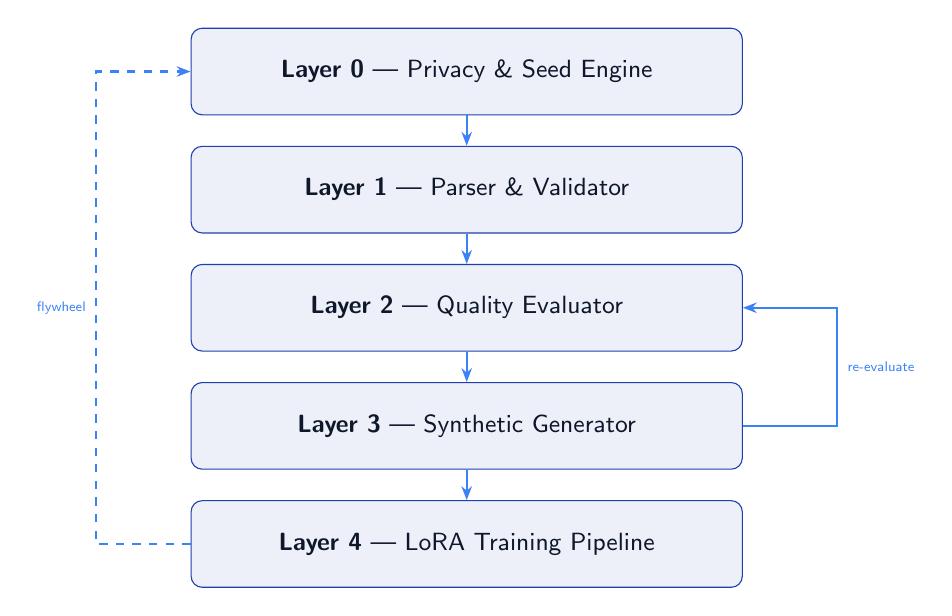
\begin{tikzpicture}[
  layer/.style={
    draw=uncaseBlue, fill=uncaseBlue!8, rounded corners=4pt,
    minimum width=7cm, minimum height=1.1cm, font=\sffamily\small,
    text=uncaseDark
  },
  arrow/.style={-{Stealth[length=5pt]}, thick, color=uncaseAccent}
]
  \node[layer] (l0) at (0,0) {\textbf{Layer 0} --- Privacy \& Seed Engine};
  \node[layer] (l1) at (0,-1.5) {\textbf{Layer 1} --- Parser \& Validator};
  \node[layer] (l2) at (0,-3) {\textbf{Layer 2} --- Quality Evaluator};
  \node[layer] (l3) at (0,-4.5) {\textbf{Layer 3} --- Synthetic Generator};
  \node[layer] (l4) at (0,-6) {\textbf{Layer 4} --- LoRA Training Pipeline};
  \draw[arrow] (l0) -- (l1);
  \draw[arrow] (l1) -- (l2);
  \draw[arrow] (l2) -- (l3);
  \draw[arrow] (l3.east) -- ++(1.2,0) |- node[right, pos=0.25, font=\sffamily\tiny\color{gray}]{re-evaluate} (l2.east);
  \draw[arrow] (l3) -- (l4);
  \draw[arrow, dashed] (l4.west) -- ++(-1.2,0) |- node[left, pos=0.25, font=\sffamily\tiny\color{gray}]{flywheel} (l0.west);
\end{tikzpicture}

\vspace{2cm}

\textcolor{gray}{\rule{8cm}{0.4pt}}\\[1em]
{\normalsize Open-source framework for generating privacy-safe synthetic\\
conversational data in regulated industries}\\[1em]
\textcolor{gray}{\rule{8cm}{0.4pt}}

\vfill

{\small\textcolor{gray}{%
\url{https://github.com/uncase-ai/uncase} \quad|\quad
\url{https://uncase.md}}}

\end{center}
\end{titlepage}

% --- Table of Contents ---
\newpage
\tableofcontents
\newpage

% =============================================================================
\section{Executive Summary}
% =============================================================================

Large language models are transforming every industry, but fine-tuning them for regulated sectors---healthcare, finance, legal, manufacturing---runs into a hard wall: \textbf{you cannot use real customer data without violating privacy regulations}, and you cannot produce high-quality domain models without real conversational patterns.

\uncase{} solves this by providing a \textbf{complete, open-source pipeline} that converts a small number of real conversation \emph{seeds}---stripped of all personally identifiable information (PII)---into thousands of synthetic training conversations that preserve the domain knowledge, tone, and structure of the originals while guaranteeing zero PII leakage.

\subsection{What UNCASE Does Today}

\begin{itemize}
  \item \textbf{5-layer pipeline} from raw data ingestion to trained LoRA adapter, fully orchestrated.
  \item \textbf{9 quality metrics} including two semantic evaluators (LLM-as-Judge and embedding drift), with hard thresholds that reject substandard data automatically.
  \item \textbf{Zero-PII guarantee}: dual-layer scanning (regex heuristics + Microsoft Presidio NER) catches 14+ categories of personal data before it enters the pipeline.
  \item \textbf{Adversarial input protection}: PromptShield module detects prompt injection, jailbreak attempts, and PII solicitation with 5 threat categories.
  \item \textbf{150 curated seed packages} across 3 industry domains (automotive, medical, finance), with 56 scenario templates covering edge cases.
  \item \textbf{11 fine-tuning export formats} (ChatML, Llama, Qwen, Mistral, and more) with full tool-call training support.
  \item \textbf{106 REST API endpoints} across 24 routers, a React 19 dashboard, a CLI, and a Python SDK.
  \item \textbf{5 compliance profiles} (HIPAA, GDPR, SOX, LFPDPPP, EU AI Act) as frozen, auditable configurations.
  \item \textbf{Enterprise-grade infrastructure}: JWT auth with RBAC, audit logging, LLM cost tracking, rate limiting, Prometheus metrics, and Grafana dashboards.
\end{itemize}

\subsection{Who Is This For}

\begin{enumerate}
  \item \textbf{ML teams in regulated industries} that need domain-specific training data without legal risk.
  \item \textbf{Enterprises deploying conversational AI} (chatbots, virtual assistants, copilots) that must comply with HIPAA, GDPR, SOX, or the EU AI Act.
  \item \textbf{AI startups} building vertical solutions that lack access to large proprietary datasets.
  \item \textbf{Data science teams} that want to augment small real-world datasets with high-quality synthetic conversations.
\end{enumerate}

% =============================================================================
\section{The Problem: Training Data in Regulated Industries}
\label{sec:problem}
% =============================================================================

\subsection{The Data Paradox}

Fine-tuning a large language model for a specific domain---say, a medical consultation assistant or a financial advisor chatbot---requires thousands of real conversations that demonstrate the correct patterns, terminology, tone, and decision-making flow.

In regulated industries, these conversations exist but are \textbf{locked behind legal, ethical, and compliance barriers}:

\begin{itemize}
  \item \textbf{HIPAA} (US): Protected Health Information cannot leave the covered entity without a Business Associate Agreement and de-identification per Safe Harbor or Expert Determination methods.
  \item \textbf{GDPR} (EU): Personal data processing requires explicit consent, purpose limitation, and data minimization. Synthetic data generation from personal data constitutes processing.
  \item \textbf{SOX} (US): Financial services must maintain audit trails for all data used in automated decision systems, with 7-year retention.
  \item \textbf{EU AI Act}: High-risk AI systems (healthcare, finance, legal) require documented training data governance, bias testing, and conformity assessments.
\end{itemize}

\subsection{Why Existing Approaches Fall Short}

\begin{table}[H]
\centering
\small
\rowcolors{2}{tableBg}{white}
\begin{tabularx}{\textwidth}{L{3cm}L{4.5cm}L{5.5cm}}
\toprule
\rowcolor{tableHeader}
\textbf{Approach} & \textbf{How It Works} & \textbf{Why It's Not Enough} \\
\midrule
Manual anonymization & Humans review and redact PII & Expensive, slow, error-prone. Misses context-dependent PII (e.g., ``the diabetic patient in room 4''). \\
Rule-based scrubbing & Regex patterns remove known PII formats & Catches emails and SSNs but misses names, locations, medical conditions embedded in free text. \\
Template generation & Fill-in-the-blank conversation templates & Produces stilted, repetitive data. Models trained on templates generate template-like output. \\
Generic LLM generation & Ask GPT-4/Claude to ``create a medical conversation'' & Lacks domain specificity. Hallucinates facts. No quality guarantees. No traceability to real patterns. \\
Data marketplaces & Buy pre-packaged datasets & Rarely domain-specific enough. Provenance unclear. May contain undetected PII. Not customizable. \\
\bottomrule
\end{tabularx}
\caption{Comparison of existing approaches to training data generation.}
\end{table}

\subsection{What's Actually Needed}

A solution that:
\begin{enumerate}
  \item Starts from \textbf{real conversational patterns} (not templates or generic prompts).
  \item Removes \textbf{all PII before any processing} begins---not after.
  \item Generates synthetic data that \textbf{preserves domain structure, tone, and factual accuracy}.
  \item \textbf{Measures quality automatically} against multiple dimensions with hard pass/fail thresholds.
  \item Produces output in \textbf{every major fine-tuning format} (ChatML, Llama, Qwen, Mistral, etc.).
  \item Maintains a \textbf{complete audit trail} from raw input to trained model.
  \item Is \textbf{open-source, self-hostable}, and runs behind the enterprise firewall.
\end{enumerate}

This is what \uncase{} provides.


% =============================================================================
\section{The SCSF Architecture}
\label{sec:architecture}
% =============================================================================

\uncase{} implements the \textbf{Synthetic Conversation Seed Framework (SCSF)}, a 5-layer pipeline where each layer has a single responsibility and communicates via validated Pydantic v2 schemas.

\subsection{Pipeline Overview}

\begin{figure}[H]
\centering
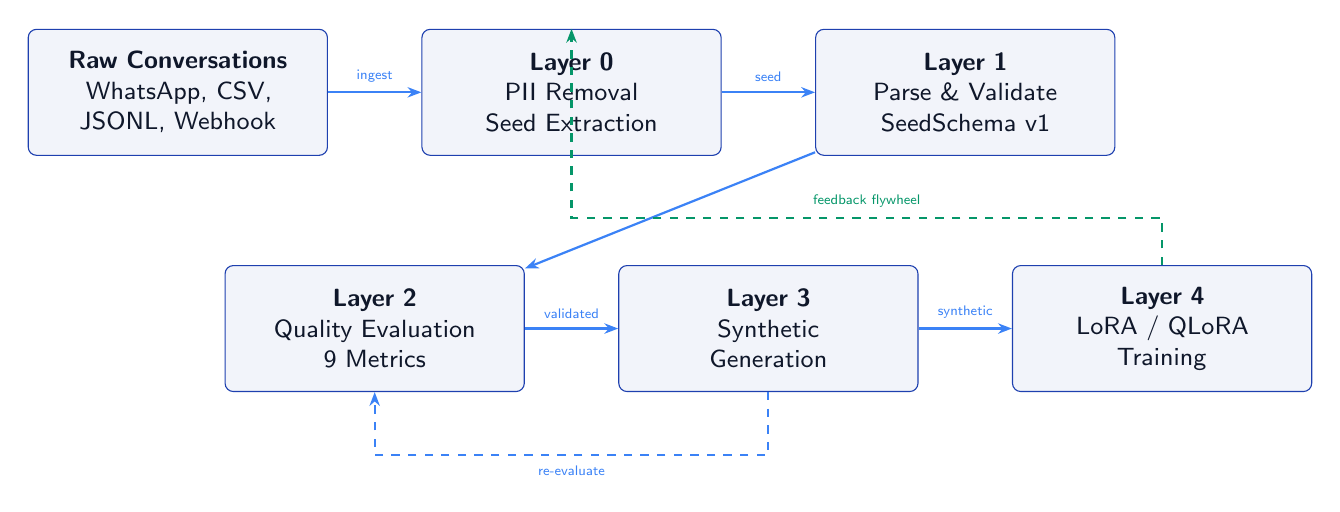
\begin{tikzpicture}[
  box/.style={draw=uncaseBlue, fill=uncaseBlue!6, rounded corners=3pt,
    minimum width=3.8cm, minimum height=1.6cm, text width=3.4cm,
    align=center, font=\sffamily\small, text=uncaseDark},
  arrow/.style={-{Stealth[length=5pt]}, thick, color=uncaseAccent},
  label/.style={font=\sffamily\tiny\color{gray}, above}
]
  % Nodes
  \node[box] (raw) at (0,0) {\textbf{Raw Conversations}\\WhatsApp, CSV,\\JSONL, Webhook};
  \node[box] (l0) at (5,0) {\textbf{Layer 0}\\PII Removal\\Seed Extraction};
  \node[box] (l1) at (10,0) {\textbf{Layer 1}\\Parse \& Validate\\SeedSchema v1};
  \node[box] (l2) at (2.5,-3) {\textbf{Layer 2}\\Quality Evaluation\\9 Metrics};
  \node[box] (l3) at (7.5,-3) {\textbf{Layer 3}\\Synthetic\\Generation};
  \node[box] (l4) at (12.5,-3) {\textbf{Layer 4}\\LoRA / QLoRA\\Training};

  % Arrows
  \draw[arrow] (raw) -- node[label]{ingest} (l0);
  \draw[arrow] (l0) -- node[label]{seed} (l1);
  \draw[arrow] (l1) -- (l2);
  \draw[arrow] (l2) -- node[label]{validated} (l3);
  \draw[arrow] (l3) -- node[label]{synthetic} (l4);

  % Re-evaluation loop
  \draw[arrow, dashed] (l3.south) -- ++(0,-0.8) -| node[below, pos=0.25, font=\sffamily\tiny\color{gray}]{re-evaluate} (l2.south);

  % Flywheel
  \draw[arrow, dashed, color=uncaseGreen] (l4.north) -- ++(0,0.6) -| node[above, pos=0.25, font=\sffamily\tiny\color{uncaseGreen}]{feedback flywheel} (l0.north);
\end{tikzpicture}
\caption{SCSF 5-layer pipeline with re-evaluation loop and feedback flywheel.}
\end{figure}

\subsection{Layer 0: Privacy \& Seed Engine}

The first layer is the \textbf{zero-trust boundary}. No raw data survives past this point.

\subsubsection{PII Detection (Dual Strategy)}

\begin{table}[H]
\centering
\small
\rowcolors{2}{tableBg}{white}
\begin{tabularx}{\textwidth}{L{3.5cm}L{2.5cm}C{2cm}L{4.5cm}}
\toprule
\rowcolor{tableHeader}
\textbf{PII Category} & \textbf{Detection} & \textbf{Token} & \textbf{Example} \\
\midrule
Email addresses & Regex & \texttt{[EMAIL]} & user@company.com \\
Phone numbers & Regex & \texttt{[PHONE]} & +52\,55\,1234\,5678 \\
SSN (US) & Regex & \texttt{[SSN]} & 123-45-6789 \\
CURP (Mexico) & Regex & \texttt{[CURP]} & GOML860101HDFRRN00 \\
RFC (Mexico) & Regex & \texttt{[RFC]} & GOML860101XXX \\
Credit cards & Regex & \texttt{[CREDIT\_CARD]} & 4111-1111-1111-1111 \\
IP addresses & Regex & \texttt{[IP\_ADDRESS]} & 192.168.1.100 \\
IBAN & Regex & \texttt{[IBAN]} & DE89370400440532013000 \\
Person names & Presidio NER & \texttt{[PERSON]} & John Smith \\
Locations & Presidio NER & \texttt{[LOCATION]} & Mexico City \\
Dates of birth & Presidio NER & \texttt{[DATE]} & 01/15/1990 \\
Medical licenses & Presidio NER & \texttt{[LICENSE]} & DEA: AB1234567 \\
Bank accounts & Presidio NER & \texttt{[BANK\_ACCT]} & Account 12345678 \\
Passport / DL & Presidio NER & \texttt{[PASSPORT]} & Passport A12345678 \\
\bottomrule
\end{tabularx}
\caption{14 PII categories detected by the dual regex + Presidio NER strategy.}
\end{table}

Regex heuristics are always active and require no external dependencies. Presidio NER (via spaCy) is an optional upgrade that catches context-dependent PII (names, locations) using named entity recognition.

\subsubsection{PromptShield: Adversarial Input Protection}

The \texttt{PromptShield} module scans all inputs \textbf{before} they reach any LLM, detecting 5 categories of adversarial content:

\begin{enumerate}
  \item \textbf{Prompt injection}: Attempts to override system instructions (``ignore all previous instructions'').
  \item \textbf{Jailbreak}: Roleplay-based bypasses (``pretend you are an unrestricted AI'').
  \item \textbf{System prompt extraction}: Requests to reveal internal configuration.
  \item \textbf{Toxic content}: Requests for harmful instructions.
  \item \textbf{PII solicitation}: Requests to bypass anonymization (``use real names'').
\end{enumerate}

Three operating modes: \texttt{audit} (log only), \texttt{warn} (log + flag), \texttt{block} (reject). An optional LLM-backed classifier provides enhanced detection for sophisticated attacks that evade regex patterns.

\subsubsection{Seed Extraction}

After PII removal, the engine extracts structural metadata from raw conversations:
\begin{itemize}
  \item \textbf{Roles}: Participants identified and labeled (e.g., ``salesperson'', ``customer'').
  \item \textbf{Domain}: Classified into one of 6 supported industry verticals.
  \item \textbf{Objective}: The purpose of the conversation inferred from content.
  \item \textbf{Tone \& style}: Formal, informal, technical, empathetic, etc.
  \item \textbf{Factual parameters}: Domain constraints, restrictions, and expected behaviors.
  \item \textbf{Expected flow}: The logical progression of conversation steps.
\end{itemize}

The output is a \texttt{SeedSchema~v1} object---a structured, validated, PII-free blueprint that drives all downstream generation.

\subsection{Layer 1: Parser \& Validator}

Accepts multiple input formats and validates them against the SeedSchema:

\begin{itemize}
  \item \textbf{WhatsApp exports} (\texttt{chat.txt}) with automatic timestamp and participant detection.
  \item \textbf{CSV transcripts} (call center format, configurable column mapping).
  \item \textbf{JSON/JSONL} (structured conversation objects).
  \item \textbf{Webhook payloads} (real-time ingestion from CRM/helpdesk systems).
\end{itemize}

All parsing produces validated Pydantic v2 models with automatic type coercion, constraint checking, and descriptive error messages.

\subsection{Layer 2: Quality Evaluator}
\label{sec:evaluator}

Every generated conversation is scored against \textbf{9 mandatory metrics}. No conversation enters the training pipeline unless it passes all thresholds.

\begin{table}[H]
\centering
\small
\rowcolors{2}{tableBg}{white}
\begin{tabularx}{\textwidth}{L{3.8cm}C{1.8cm}C{1.2cm}L{5.2cm}}
\toprule
\rowcolor{tableHeader}
\textbf{Metric} & \textbf{Threshold} & \textbf{Gate?} & \textbf{What It Measures} \\
\midrule
ROUGE-L & $\geq 0.65$ & No & Structural coherence with the seed \\
Factual Fidelity & $\geq 0.90$ & No & Domain fact accuracy \\
Lexical Diversity (TTR) & $\geq 0.55$ & No & Vocabulary richness (type-token ratio) \\
Dialogic Coherence & $\geq 0.85$ & No & Inter-turn logical consistency \\
Tool Call Validity & $\geq 0.90$ & No & Tool call schema correctness (5 dimensions) \\
Semantic Fidelity & $\geq 0.60$ & No & LLM-as-Judge rubric score (4 dimensions) \\
Embedding Drift & $\geq 0.40$ & No & Cosine similarity between seed and generated text \\
Privacy Score & $= 0.00$ & \textbf{Yes} & Zero residual PII (hard gate) \\
Memorization & $< 0.01$ & \textbf{Yes} & Extraction attack success rate (hard gate) \\
\bottomrule
\end{tabularx}
\caption{Quality metrics with mandatory thresholds. Gate metrics cause immediate rejection.}
\end{table}

\subsubsection{Composite Score Formula}

\begin{equation}
Q = \begin{cases}
\min(\text{ROUGE-L}, \text{Fidelity}, \text{TTR}, \text{Coherence}, \text{Tool Validity}, \text{Sem. Fidelity}, \text{Emb. Drift})
  & \text{if } \text{privacy} = 0 \text{ and } \text{memorization} < 0.01 \\
0 & \text{otherwise}
\end{cases}
\end{equation}

Using the \textbf{minimum} rather than the average ensures no single dimension can be weak while others compensate. The privacy and memorization metrics act as hard gates: any PII leakage or memorization above threshold sets $Q = 0$ regardless of other scores.

\subsubsection{Semantic Fidelity (LLM-as-Judge)}

A fast, cost-efficient LLM (default: Claude Haiku) grades each conversation on a structured rubric across 4 dimensions:

\begin{enumerate}
  \item \textbf{Factual fidelity} (35\% weight): Does it respect domain constraints?
  \item \textbf{Logical coherence} (30\%): Does the dialog flow make sense?
  \item \textbf{Role consistency} (20\%): Do participants stay in character?
  \item \textbf{Naturalness} (15\%): Does it feel like a real conversation?
\end{enumerate}

Each dimension is graded 1--5, then the weighted average is normalized to $[0, 1]$. The metric falls back gracefully to a neutral score (0.5) when the LLM API is unavailable.

\subsubsection{Embedding Drift}

Measures semantic distance between the seed specification and the generated conversation using cosine similarity over embedding vectors. High similarity means the conversation stays on-topic; low similarity indicates drift.

Two backends:
\begin{itemize}
  \item \textbf{LLM embeddings} (primary): Uses provider-agnostic embedding API via LiteLLM.
  \item \textbf{TF-IDF fallback} (always available): Term-frequency cosine similarity, no API required.
\end{itemize}

\subsubsection{Tool Call Validator}

For conversations involving tool use, a dedicated validator checks 5 dimensions:
\begin{enumerate}
  \item \textbf{Hallucinated tools}: Tool name doesn't exist in the seed's definitions.
  \item \textbf{Missing required arguments}: Required parameters not provided.
  \item \textbf{Unknown arguments}: Parameters not defined in the tool schema.
  \item \textbf{Type mismatches}: Argument types don't match schema definitions.
  \item \textbf{Sequence validation}: Tool call order matches expected patterns (exact, subset, or partial order).
\end{enumerate}


\subsection{Layer 3: Synthetic Generator}

The generation engine uses \textbf{LiteLLM} as a provider-agnostic interface, supporting 7+ LLM providers:

\begin{table}[H]
\centering
\small
\rowcolors{2}{tableBg}{white}
\begin{tabularx}{\textwidth}{L{3.5cm}L{2.5cm}L{6cm}}
\toprule
\rowcolor{tableHeader}
\textbf{Provider} & \textbf{Connection} & \textbf{Example Models} \\
\midrule
Anthropic (Claude) & Cloud API & Claude Sonnet 4.6, Claude Haiku 4.5 \\
OpenAI & Cloud API & GPT-4o, GPT-4o-mini \\
Google (Gemini) & Cloud API & Gemini 2.0 Flash, Gemini 2.5 Pro \\
Groq & Cloud API & Llama 3.3-70B, Mixtral 8x7B \\
Ollama & Local API & Any GGUF model \\
vLLM & Local API & Any HuggingFace model \\
Custom (OpenAI-compatible) & Any & Together AI, Fireworks, etc. \\
\bottomrule
\end{tabularx}
\caption{Supported LLM providers via LiteLLM.}
\end{table}

\subsubsection{Smart Retry Strategy}

The generator implements an intelligent retry mechanism:

\begin{enumerate}
  \item First attempt uses \texttt{response\_format=json\_object} when the model supports it.
  \item On JSON format failure, retries without structured output.
  \item On each retry, \textbf{escalates temperature} by a configurable step (default: +0.1) to encourage diverse output and escape degenerate patterns.
  \item Structured JSON extraction uses direct parse, markdown code block extraction, and object-key unwrapping---but \textbf{no fragile regex bracket-matching} that could silently corrupt data.
\end{enumerate}

\subsubsection{Feedback-Augmented Generation}

When a conversation fails quality evaluation, the generator receives specific feedback about which metrics failed and by how much. The next generation attempt incorporates this feedback as additional prompt instructions, creating a \textbf{self-correcting loop} between Layers 2 and 3.

\subsubsection{Parallel Pipeline Orchestration}

The pipeline orchestrator uses \texttt{asyncio.gather()} with \textbf{semaphore-based concurrency control} to process seeds and conversations in parallel while respecting LLM rate limits. Configurable concurrency (default: 10 concurrent operations) prevents overwhelming API rate limits while maximizing throughput.

Three stages run in parallel:
\begin{enumerate}
  \item \textbf{Seed creation}: Multiple raw conversations processed concurrently.
  \item \textbf{Generation}: Multiple seeds generate synthetic data simultaneously.
  \item \textbf{Evaluation}: Batched concurrent evaluation with configurable batch sizes.
\end{enumerate}


\subsection{Layer 4: LoRA Training Pipeline}

The final layer transforms certified synthetic data into trained model adapters:

\begin{itemize}
  \item \textbf{LoRA/QLoRA fine-tuning} via HuggingFace Transformers + PEFT.
  \item \textbf{11 export formats} ensure compatibility with every major model architecture.
  \item \textbf{MLflow experiment tracking} for hyperparameter logging and model versioning.
  \item \textbf{GPU deployment scripts} for vLLM serving with tensor parallelism (A40, A100, H100).
  \item Merge and serve pipeline: download base model, apply LoRA adapter, serve via vLLM with Cloudflare Tunnel for public access.
\end{itemize}

\begin{table}[H]
\centering
\small
\rowcolors{2}{tableBg}{white}
\begin{tabularx}{\textwidth}{L{3cm}C{2.5cm}L{7cm}}
\toprule
\rowcolor{tableHeader}
\textbf{Format} & \textbf{Tool Support} & \textbf{Compatible Models} \\
\midrule
ChatML & \cmark & GPT-4, Qwen (base), Yi \\
Llama 3/4 & \cmark & LLaMA 3, 3.1, 4 \\
Qwen 3 & \cmark & Qwen 3, Qwen 2.5 \\
Mistral & \cmark & Mistral, Mixtral \\
Nemotron & \cmark & NVIDIA Nemotron \\
Harmony & \cmark & Cohere Command R+ \\
Kimi/Moonshot & \cmark & Moonshot Kimi \\
MiniMax & \cmark & MiniMax \\
OpenAI API & \cmark & Any OpenAI-compatible endpoint \\
Alpaca & \xmark & Instruction-tuned models \\
\bottomrule
\end{tabularx}
\caption{Supported fine-tuning export formats. All formats except Alpaca support tool-use training data.}
\end{table}


% =============================================================================
\section{Domain Coverage \& Scenario Templates}
\label{sec:domains}
% =============================================================================

\subsection{150 Curated Seed Packages}

\uncase{} ships with \textbf{150 professionally curated conversation seeds} across 3 primary domains, with 3 additional domains supported via scenario templates:

\begin{table}[H]
\centering
\small
\rowcolors{2}{tableBg}{white}
\begin{tabularx}{\textwidth}{L{3.5cm}C{1.5cm}C{2cm}L{5.5cm}}
\toprule
\rowcolor{tableHeader}
\textbf{Domain} & \textbf{Seeds} & \textbf{Scenarios} & \textbf{Key Topics} \\
\midrule
Automotive Sales & 50 & 12 + 5 edge & Vehicle inquiry, test drives, financing, trade-ins, fleet sales, warranty, frustrated customer \\
Medical Consultation & 50 & 10 + 3 edge & Patient history, symptom assessment, lab results, prescriptions, insurance, anxious patient \\
Finance Advisory & 50 & 10 + 4 edge & Portfolio review, risk profiling, market panic, suspicious activity, KYC/AML \\
Legal Advisory & --- & 8 + 3 edge & Case intake, conflict of interest, scope limitation, fee structures \\
Industrial Support & --- & 8 + 3 edge & Equipment diagnostics, safety incidents, production down, parts ordering \\
Education Tutoring & --- & 8 + 3 edge & Concept explanation, frustrated student, learning styles, exam prep \\
\bottomrule
\end{tabularx}
\caption{Domain coverage with curated seeds and scenario templates.}
\end{table}

\subsection{Scenario Template System}

Each scenario template defines:
\begin{itemize}
  \item \textbf{Intent and objective}: What the conversation should accomplish.
  \item \textbf{Skill level}: Basic, intermediate, or advanced complexity.
  \item \textbf{Expected tool sequence}: Which domain tools should be called and in what order.
  \item \textbf{Flow steps}: Logical progression that overrides the seed's default flow.
  \item \textbf{Edge-case flag}: Marks scenarios that stress-test model robustness.
  \item \textbf{Weighted random selection}: Control scenario distribution in batch generation.
\end{itemize}

\subsection{30 Domain Tools (5 per Industry)}

Each domain comes with 5 built-in tools that simulate real-world integrations:

\begin{table}[H]
\centering
\small
\rowcolors{2}{tableBg}{white}
\begin{tabularx}{\textwidth}{L{2.5cm}L{10cm}}
\toprule
\rowcolor{tableHeader}
\textbf{Domain} & \textbf{Tools} \\
\midrule
Automotive & Inventory search, price quotes, financing calculator, model comparison, CRM lookup \\
Medical & Patient history, medication database, appointments, lab results, insurance verification \\
Finance & Portfolio analysis, risk profiles, market data, KYC/AML checks, scenario simulation \\
Legal & Case law search, case files, court deadlines, legislation lookup, fee calculator \\
Industrial & Equipment diagnostics, parts inventory, maintenance scheduling, safety reporting \\
Education & Curriculum search, progress tracking, exercise generator, resource library, scheduling \\
\bottomrule
\end{tabularx}
\caption{Built-in domain tools for tool-use training data generation.}
\end{table}


% =============================================================================
\section{Privacy \& Compliance Framework}
\label{sec:privacy}
% =============================================================================

\subsection{Design Principle: Privacy by Architecture}

\uncase{} does not attempt to ``anonymize data well enough.'' Instead, it ensures \textbf{real data never reaches the generation or training stages}:

\begin{enumerate}
  \item \textbf{Ingest}: Raw conversations enter Layer 0.
  \item \textbf{Scan}: Dual-layer PII detection (regex + NER) identifies all personal data.
  \item \textbf{Replace}: PII tokens replace real data (\texttt{[PERSON]}, \texttt{[EMAIL]}, etc.).
  \item \textbf{Extract}: Structural metadata is extracted into a SeedSchema---a blueprint, not data.
  \item \textbf{Generate}: Layer 3 creates entirely new conversations from the blueprint.
  \item \textbf{Verify}: Layer 2 re-scans generated output, rejecting anything with residual PII.
\end{enumerate}

The generated synthetic conversations \textbf{never contained real PII in the first place}---they were created from anonymized blueprints. This is fundamentally different from generating data and then trying to remove PII afterward.

\subsection{Privacy Gateway}

The LLM Gateway intercepts all messages going to and from external LLM providers, scanning for PII in three modes:

\begin{itemize}
  \item \texttt{audit}: Scan and log detections (for monitoring).
  \item \texttt{warn}: Scan, log, and include warnings in the API response.
  \item \texttt{block}: Reject any request or response containing PII.
\end{itemize}

All provider API keys are \textbf{Fernet-encrypted at rest} in the database.

\subsection{Compliance Profiles}

Five regulatory frameworks are implemented as \textbf{frozen dataclass configurations}---immutable, auditable, version-controlled:

\begin{table}[H]
\centering
\small
\rowcolors{2}{tableBg}{white}
\begin{tabularx}{\textwidth}{L{2cm}C{1.5cm}C{1.5cm}C{2cm}L{5cm}}
\toprule
\rowcolor{tableHeader}
\textbf{Profile} & \textbf{PII Types} & \textbf{$\epsilon$ (DP)} & \textbf{Retention} & \textbf{Key Requirements} \\
\midrule
HIPAA & 21 & $\leq 3.0$ & 7 years & RBAC + MFA, BAA, Safe Harbor \\
GDPR & 17 & $\leq 5.0$ & 1 year & Right to erasure, DPIA, portability \\
SOX & 9 & $\leq 5.0$ & 7 years & Audit trail, segregation of duties \\
LFPDPPP & 10 & Optional & 1 year & ARCO rights (Mexico) \\
EU AI Act & 7 & $\leq 5.0$ & --- & Risk classification, Art.~11 documentation \\
\bottomrule
\end{tabularx}
\caption{Compliance profile configurations with PII categories, differential privacy budgets, and retention policies.}
\end{table}

Each profile specifies:
\begin{itemize}
  \item Which PII categories must be detected and removed.
  \item Differential privacy epsilon budget for fine-tuning.
  \item Data retention periods and auto-deletion schedules.
  \item Quality metric thresholds (stricter for higher-risk domains).
  \item Required access control and audit mechanisms.
\end{itemize}


% =============================================================================
\section{Enterprise Infrastructure}
\label{sec:enterprise}
% =============================================================================

\subsection{API Architecture}

The \uncase{} backend exposes \textbf{106 REST API endpoints} across \textbf{24 routers}, built on FastAPI with async PostgreSQL (via asyncpg + SQLAlchemy):

\begin{table}[H]
\centering
\small
\rowcolors{2}{tableBg}{white}
\begin{tabularx}{\textwidth}{L{3.5cm}C{2cm}L{7cm}}
\toprule
\rowcolor{tableHeader}
\textbf{Category} & \textbf{Endpoints} & \textbf{Capabilities} \\
\midrule
Authentication & 3 & JWT login, token refresh, verification \\
Organizations & 7 & CRUD, members, settings, API keys \\
Seeds & 6 & CRUD, batch operations, domain filtering \\
Generation & 1 & Seed-guided synthetic conversation creation \\
Evaluation & 4 & Single/batch evaluation, quality reports \\
Templates & 5 & 11 format renderers, preview, conversion \\
Tools & 8 & CRUD, execution, simulation, search \\
Providers & 6 & LLM provider CRUD, connection testing \\
Connectors & 8 & WhatsApp, webhook, PII scan, imports \\
Gateway & 2 & Privacy-intercepted LLM chat \\
Sandbox & 5 & E2B code execution, demos, Opik eval \\
Plugins & 7 & Install, uninstall, registry, marketplace \\
Pipeline & 1 & End-to-end orchestration \\
Jobs & 3 & Background job queue, cancel \\
Knowledge & 5 & Document upload, vector search \\
Usage & 4 & Metering, analytics, cost breakdown \\
Webhooks & 8 & Subscriptions, deliveries, retry \\
Audit & 1 & Compliance trail, export \\
Costs & 3 & LLM spend per org/job \\
Health & 3 & Liveness, readiness, deep checks \\
\bottomrule
\end{tabularx}
\caption{API endpoint summary by category.}
\end{table}

\subsection{Authentication \& Authorization}

\begin{itemize}
  \item \textbf{JWT access + refresh token pair} with configurable expiration and rotation.
  \item \textbf{Role-Based Access Control (RBAC)}: Admin, Developer, Viewer roles per organization.
  \item \textbf{Organization-scoped isolation}: All queries filtered by \texttt{org\_id}.
  \item \textbf{API key authentication}: Fernet-encrypted keys with scoped permissions.
  \item \textbf{Argon2 password hashing} (memory-hard, timing-safe).
\end{itemize}

\subsection{Audit Logging}

An immutable compliance trail records:
\begin{itemize}
  \item Who accessed what data, when, and from where (IP, user agent).
  \item All CRUD operations on seeds, conversations, providers, and organization settings.
  \item Authentication events (login, logout, token refresh, failed attempts).
  \item Pipeline runs with full input/output metadata.
\end{itemize}

Audit logs are stored in a dedicated PostgreSQL table (\texttt{audit\_logs}) with separate retention from application data.

\subsection{Rate Limiting}

Per-key sliding window rate limiting with 4 tiers:

\begin{table}[H]
\centering
\small
\rowcolors{2}{tableBg}{white}
\begin{tabularx}{\textwidth}{L{3cm}C{3cm}L{6cm}}
\toprule
\rowcolor{tableHeader}
\textbf{Tier} & \textbf{Requests/min} & \textbf{Target} \\
\midrule
Free & 60 & Open-source users, evaluation \\
Developer & 300 & Active development, testing \\
Enterprise & 1,000 & Production workloads \\
Default & 120 & Unclassified API keys \\
\bottomrule
\end{tabularx}
\caption{Rate limit tiers.}
\end{table}

Two backends: in-memory sliding window (single instance) and Redis sorted sets (distributed). Automatic fallback to in-memory when Redis is unavailable. Returns standard \texttt{429 Too Many Requests} with \texttt{Retry-After} header.

\subsection{Observability}

\begin{itemize}
  \item \textbf{Prometheus metrics} at \texttt{/metrics}: request rate, latency (avg, p95, p99), error rate, database query duration, LLM API latency.
  \item \textbf{Pre-built Grafana dashboard} (included in repository): real-time monitoring of all API and infrastructure metrics.
  \item \textbf{Structured logging} via structlog (JSON format) with contextual fields (seed ID, domain, organization, etc.).
  \item \textbf{Usage metering}: Fire-and-forget event recording for analytics and billing.
  \item \textbf{LLM cost tracking}: Per-organization and per-job spend tracking for all LLM API calls.
\end{itemize}

\subsection{Background Job System}

Long-running operations (generation, evaluation, training) run as background jobs with:
\begin{itemize}
  \item Job submission via API with unique job IDs.
  \item Real-time progress tracking (percentage, stage, estimated completion).
  \item Cancellation support.
  \item Automatic retry with exponential backoff.
  \item Job history and result storage in PostgreSQL.
\end{itemize}


% =============================================================================
\section{Dashboard \& Developer Experience}
\label{sec:dashboard}
% =============================================================================

\subsection{Web Dashboard}

A full-featured React 19 dashboard (Next.js 16, TypeScript, shadcn/ui, Tailwind CSS 4) provides a visual interface for the entire pipeline:

\begin{table}[H]
\centering
\small
\rowcolors{2}{tableBg}{white}
\begin{tabularx}{\textwidth}{L{3cm}L{9.5cm}}
\toprule
\rowcolor{tableHeader}
\textbf{Page} & \textbf{Functionality} \\
\midrule
Overview & Pipeline status, key metrics, recent activity at a glance \\
Pipeline & Seed-to-model workflow wizard with step-by-step progress \\
Conversations & Browse, search, and inspect generated synthetic conversations \\
Templates & Select and preview fine-tuning export formats \\
Tools & Browse, create, and test domain tools \\
Evaluations & Quality metric reports with drill-down by metric \\
Knowledge & Upload and search knowledge base documents \\
Activity & Audit log browser with filtering \\
Settings & Organization configuration, members, API keys \\
Plugins & Plugin marketplace, install/uninstall, per-domain packs \\
Jobs & Background job queue with real-time status \\
Costs & LLM API spend tracking per organization and per job \\
\bottomrule
\end{tabularx}
\caption{Dashboard pages and their functionality.}
\end{table}

\subsection{CLI}

A Typer-based CLI provides full pipeline access from the terminal:

\begin{lstlisting}[language=bash]
# Create a seed from a raw conversation
uncase seed create --domain automotive.sales --file chat.txt

# Generate 1,000 synthetic conversations
uncase generate --seed-id abc123 --count 1000 --model gemini-2.0-flash

# Evaluate quality
uncase evaluate --conversation-id xyz789

# Run the full pipeline
uncase pipeline run --domain medical.consultation --count 500

# Export to Llama format
uncase template render --format llama --output training_data.jsonl
\end{lstlisting}

\subsection{Python SDK}

For programmatic access, the SDK provides 6 wrapper classes:

\begin{lstlisting}[language=Python]
from uncase import Pipeline, SeedEngine, Generator, Evaluator

# End-to-end pipeline
pipeline = Pipeline(api_url="http://localhost:8000")
result = pipeline.run(
    domain="automotive.sales",
    raw_conversations=["chat1.txt", "chat2.txt"],
    count=1000,
    model="claude-sonnet-4-6",
)

# Or use individual components
engine = SeedEngine()
seed = engine.create_seed(raw_text, domain="medical.consultation")
generator = Generator(model="gemini-2.0-flash")
conversations = generator.generate(seed, count=100)
evaluator = Evaluator()
reports = evaluator.evaluate_batch(conversations, seed)
\end{lstlisting}


% =============================================================================
\section{Deployment Options}
\label{sec:deployment}
% =============================================================================

\subsection{Three Installation Paths}

\begin{table}[H]
\centering
\small
\rowcolors{2}{tableBg}{white}
\begin{tabularx}{\textwidth}{L{3cm}L{4cm}L{5.5cm}}
\toprule
\rowcolor{tableHeader}
\textbf{Method} & \textbf{Command} & \textbf{Best For} \\
\midrule
Git + uv & \texttt{git clone \&\& uv sync} & Development, contribution \\
pip & \texttt{pip install uncase[all]} & Integration into existing projects \\
Docker & \texttt{docker compose up -d} & Production deployment \\
\bottomrule
\end{tabularx}
\caption{Installation methods.}
\end{table}

\subsection{Docker Compose Services}

\begin{table}[H]
\centering
\small
\rowcolors{2}{tableBg}{white}
\begin{tabularx}{\textwidth}{L{2.5cm}C{1.2cm}L{2cm}L{6cm}}
\toprule
\rowcolor{tableHeader}
\textbf{Service} & \textbf{Port} & \textbf{Profile} & \textbf{Purpose} \\
\midrule
api & 8000 & default & FastAPI REST API \\
postgres & 5433 & default & PostgreSQL 16 (primary datastore) \\
redis & 6379 & default & Rate limiting, caching \\
dashboard & 3000 & default & React 19 web UI \\
mlflow & 5000 & \texttt{ml} & ML experiment tracking \\
api-gpu & 8001 & \texttt{gpu} & GPU-accelerated API (NVIDIA CUDA) \\
prometheus & 9090 & \texttt{observability} & Metrics collection \\
grafana & 3001 & \texttt{observability} & Dashboards \& alerting \\
\bottomrule
\end{tabularx}
\caption{Docker Compose services and profiles.}
\end{table}

\begin{lstlisting}[language=bash]
# Standard deployment (API + DB + Redis + Dashboard)
docker compose up -d

# With ML tracking
docker compose --profile ml up -d

# With GPU support
docker compose --profile gpu up -d

# Full observability stack
docker compose --profile observability up -d
\end{lstlisting}

\subsection{GPU Deployment for Fine-Tuned Models}

Production deployment scripts support:
\begin{itemize}
  \item \textbf{Auto-detection}: Identifies GPU type (A40, A100, H100, RTX 5090) and configures memory limits automatically.
  \item \textbf{Tensor parallelism}: Distributes models across multiple GPUs for larger models (32B+).
  \item \textbf{LoRA merge pipeline}: Downloads base model + LoRA adapter, merges weights, and serves via vLLM.
  \item \textbf{Cloudflare Tunnel}: Optional public access via fixed domain (e.g., \texttt{api.domain.com}).
  \item \textbf{Health monitoring}: Automatic service health checks with retry logic and graceful shutdown.
\end{itemize}


% =============================================================================
\section{Codebase Metrics}
\label{sec:metrics}
% =============================================================================

\begin{table}[H]
\centering
\small
\rowcolors{2}{tableBg}{white}
\begin{tabularx}{\textwidth}{L{5cm}R{3cm}L{4.5cm}}
\toprule
\rowcolor{tableHeader}
\textbf{Metric} & \textbf{Value} & \textbf{Notes} \\
\midrule
Python source files & 203 & Backend framework \\
Python LOC & 36,638 & Excluding tests \\
TypeScript/React components & 132 & Dashboard frontend \\
Frontend LOC & 62,200 & TS/TSX combined \\
API endpoints & 106 & Across 24 routers \\
Pydantic models & 93 & Data validation \\
SQLAlchemy models & 18 & Database schema \\
Alembic migrations & 13 & Schema evolution \\
Test files & 80 & Unit + integration + privacy \\
Test functions & 1,160 & Automated test cases \\
Compliance profiles & 5 & HIPAA, GDPR, SOX, LFPDPPP, AI Act \\
Curated seeds & 150 & 3 domains (50 each) \\
Scenario templates & 56 & 6 industry verticals \\
Domain tools & 30 & 5 per industry \\
Export formats & 11 & Fine-tuning templates \\
Official plugins & 6 & One per industry \\
SDK wrapper classes & 6 & Programmatic API \\
Docker services & 8 & 3 optional profiles \\
\bottomrule
\end{tabularx}
\caption{Current codebase metrics as of March 2026.}
\end{table}


% =============================================================================
\section{Use Cases}
\label{sec:usecases}
% =============================================================================

\subsection{Automotive: Dealership AI Assistant}

\textbf{Problem}: A national dealership network wants to fine-tune a conversational AI assistant for their sales team, trained on patterns from their best-performing salespeople. Their CRM contains 50,000+ real customer conversations that cannot leave the dealership's infrastructure due to financial data regulations.

\textbf{UNCASE Solution}:
\begin{enumerate}
  \item Export 500 representative conversations from the CRM.
  \item UNCASE Layer 0 strips all customer PII and creates 500 seeds.
  \item Layer 3 generates 10,000 synthetic conversations, each maintaining the sales methodology and domain knowledge.
  \item Layer 2 evaluates quality (ROUGE-L, factual fidelity, tool-call correctness for inventory/pricing tools).
  \item Layer 4 produces a LoRA adapter fine-tuned on Qwen 3-14B.
  \item Deploy via vLLM with the included GPU scripts.
\end{enumerate}

\textbf{Result}: Domain-specific AI assistant trained on realistic patterns, zero customer data exposure, full audit trail for compliance.

\subsection{Healthcare: Medical Consultation Training}

\textbf{Problem}: A health-tech startup needs to train a triage assistant that handles patient intake calls. HIPAA requires that no Protected Health Information (PHI) is used in model training without formal de-identification.

\textbf{UNCASE Solution}:
\begin{enumerate}
  \item Use the HIPAA compliance profile ($\epsilon \leq 3.0$, 21 PHI categories).
  \item Import anonymized consultation transcripts via the WhatsApp/CSV connectors.
  \item Generate 5,000 synthetic consultations with the medical domain seed package (50 seeds, 10 scenario templates).
  \item Semantic fidelity ensures medical terminology and triage protocols are preserved.
  \item Export in Llama 4 format for fine-tuning.
\end{enumerate}

\subsection{Finance: Compliance-Safe Advisor Training}

\textbf{Problem}: A wealth management firm needs conversational AI for portfolio reviews and risk assessments. SOX and GDPR require 7-year audit trails and strict data governance.

\textbf{UNCASE Solution}:
\begin{enumerate}
  \item Use SOX + GDPR compliance profiles simultaneously (intersect requirements).
  \item Import advisor-client conversations with financial PII removal (9 categories including SSN, bank accounts, credit cards).
  \item Generate synthetic conversations with the finance domain pack, including KYC/AML and market panic edge-case scenarios.
  \item Audit logging captures every step for SOX compliance.
  \item Cost tracking monitors LLM API spend per training run.
\end{enumerate}


% =============================================================================
\section{Competitive Positioning}
\label{sec:competitive}
% =============================================================================

\begin{table}[H]
\centering
\small
\rowcolors{2}{tableBg}{white}
\begin{tabularx}{\textwidth}{L{3.5cm}C{1.6cm}C{1.6cm}C{1.6cm}C{1.6cm}C{1.6cm}}
\toprule
\rowcolor{tableHeader}
\textbf{Capability} & \textbf{UNCASE} & \textbf{Gretel} & \textbf{Mostly AI} & \textbf{Tonic} & \textbf{DIY Scripts} \\
\midrule
\footnotesize Conversational data focus & \cmark & \xmark & \xmark & \xmark & Partial \\
\footnotesize Multi-industry seeds & \cmark & \xmark & \xmark & \xmark & \xmark \\
\footnotesize 9 quality metrics & \cmark & Partial & \xmark & \xmark & \xmark \\
\footnotesize LLM-as-Judge eval & \cmark & \xmark & \xmark & \xmark & \xmark \\
\footnotesize Tool-use training data & \cmark & \xmark & \xmark & \xmark & \xmark \\
\footnotesize 11 export formats & \cmark & \xmark & \xmark & \xmark & Manual \\
\footnotesize Compliance profiles & \cmark & Partial & Partial & \cmark & \xmark \\
\footnotesize Open source & \cmark & \xmark & \xmark & \xmark & \cmark \\
\footnotesize Self-hostable & \cmark & \xmark & \xmark & \xmark & \cmark \\
\footnotesize Built-in LoRA pipeline & \cmark & \xmark & \xmark & \xmark & Manual \\
\bottomrule
\end{tabularx}
\caption{Competitive comparison. UNCASE is the only solution purpose-built for synthetic conversational training data in regulated industries.}
\end{table}

\textbf{Key differentiators}:
\begin{enumerate}
  \item \textbf{Conversation-native}: Built from the ground up for multi-turn dialog, not tabular data.
  \item \textbf{Seed-based generation}: Preserves real-world patterns without exposing real data.
  \item \textbf{Quality-first}: 9 metrics with hard thresholds---no conversation reaches training without certification.
  \item \textbf{Compliance-ready}: 5 regulatory profiles, audit logging, encryption at rest.
  \item \textbf{Open source}: Full transparency, self-hostable, no vendor lock-in.
  \item \textbf{End-to-end}: From raw conversations to trained LoRA adapter in a single pipeline.
\end{enumerate}


% =============================================================================
\section{Roadmap}
\label{sec:roadmap}
% =============================================================================

\begin{table}[H]
\centering
\small
\rowcolors{2}{tableBg}{white}
\begin{tabularx}{\textwidth}{C{2cm}L{4cm}L{6.5cm}}
\toprule
\rowcolor{tableHeader}
\textbf{Timeline} & \textbf{Milestone} & \textbf{Description} \\
\midrule
Q1 2026 & \textcolor{uncaseGreen}{Completed} & 5-layer pipeline, 106 endpoints, 150 seeds, 5 compliance profiles, semantic evaluation, prompt shield, parallel pipeline, GPU deployment \\
Q2 2026 & Formal DP-SGD & Opacus integration with certified epsilon accounting during fine-tuning \\
Q2 2026 & Benchmark publication & Validation against public conversation datasets with reproducible results \\
Q2 2026 & Model marketplace & Share trained LoRA adapters (not data) between organizations \\
Q3 2026 & Additional domains & Real estate, insurance, customer service, e-commerce seed packages \\
Q3 2026 & SOC 2 Type I & Security audit and compliance certification \\
Q4 2026 & Multi-modal support & Image + text conversation training data \\
Q4 2026 & Kubernetes operator & Native K8s deployment with auto-scaling \\
\bottomrule
\end{tabularx}
\caption{Development roadmap.}
\end{table}


% =============================================================================
\section{Technical Stack Summary}
\label{sec:stack}
% =============================================================================

\begin{table}[H]
\centering
\small
\rowcolors{2}{tableBg}{white}
\begin{tabularx}{\textwidth}{L{3.5cm}L{4cm}L{5cm}}
\toprule
\rowcolor{tableHeader}
\textbf{Component} & \textbf{Technology} & \textbf{Purpose} \\
\midrule
Language (backend) & Python $\geq$ 3.11 & Core framework \\
Language (frontend) & TypeScript 5.9 (strict) & Dashboard UI \\
API framework & FastAPI + Uvicorn & Async REST API \\
Frontend framework & Next.js 16, React 19 & Dashboard \& landing page \\
UI components & shadcn/ui + Radix UI & Accessible component library \\
Styling & Tailwind CSS 4 & Utility-first CSS \\
Validation & Pydantic v2 & Schema enforcement \\
Database & PostgreSQL 16 (async) & Primary datastore \\
Cache / Rate limit & Redis 7 & Distributed rate limiting \\
ORM & SQLAlchemy 2.0 (async) & Database access \\
Migrations & Alembic & Schema evolution \\
LLM interface & LiteLLM & Provider-agnostic LLM calls \\
ML training & Transformers + PEFT + TRL & LoRA fine-tuning \\
ML tracking & MLflow & Experiment logging \\
PII detection & Presidio + spaCy & Named entity recognition \\
Logging & structlog & JSON structured logging \\
CLI & Typer & Command-line interface \\
Monitoring & Prometheus + Grafana & Metrics \& dashboards \\
Containerization & Docker Compose & Multi-service deployment \\
Model serving & vLLM & GPU inference server \\
Security & Fernet, Argon2, PyJWT & Encryption, hashing, auth \\
\bottomrule
\end{tabularx}
\caption{Complete technology stack.}
\end{table}


% =============================================================================
\section{Getting Started}
\label{sec:quickstart}
% =============================================================================

\begin{lstlisting}[language=bash]
# Clone and install
git clone https://github.com/uncase-ai/uncase.git
cd uncase && uv sync --extra all

# Start the API + database
docker compose up -d

# Run the pipeline with curated seeds
uv run uncase pipeline run \
  --domain automotive.sales \
  --count 1000 \
  --model gemini-2.0-flash

# Or use pip
pip install "uncase[all]"
\end{lstlisting}

Full documentation: \url{https://uncase.md} \\
Source code: \url{https://github.com/uncase-ai/uncase} \\
API reference: \url{https://app.uncase.md/docs}


% =============================================================================
\section{Conclusion}
\label{sec:conclusion}
% =============================================================================

The adoption of AI in regulated industries is constrained not by model capability, but by \textbf{the availability of safe, high-quality training data}. Organizations that need domain-specific conversational AI are caught between the legal impossibility of using real customer data and the inadequacy of generic synthetic data.

\uncase{} resolves this tension with a principled, layered architecture:
\begin{enumerate}
  \item Real conversations are \textbf{never used directly}---only their structural blueprints survive past the privacy boundary.
  \item Every piece of generated data is \textbf{automatically evaluated} against 9 quality dimensions with hard rejection thresholds.
  \item The entire pipeline---from ingestion to trained model---is \textbf{auditable, reproducible, and compliant} with 5 major regulatory frameworks.
  \item The system is \textbf{open-source and self-hostable}, eliminating vendor lock-in and enabling deployment behind enterprise firewalls.
\end{enumerate}

With 203 Python source files, 106 API endpoints, 1,160 automated tests, 150 curated domain seeds, and 5 compliance profiles already implemented, \uncase{} is production-ready infrastructure for the next generation of privacy-safe, domain-specific AI.

\vfill

\begin{center}
\textcolor{gray}{\rule{8cm}{0.4pt}}\\[1em]
{\small\textcolor{gray}{%
UNCASE is open source under the MIT license.\\
\url{https://github.com/uncase-ai/uncase}}}
\end{center}


\end{document}
